\documentclass[tikz]{standalone}
\usetikzlibrary{decorations.pathreplacing}
\begin{document}
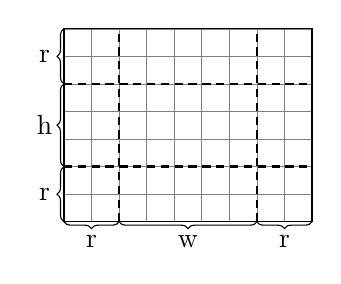
\begin{tikzpicture}[scale=0.35]
  % Drawing parameters
  \pgfmathsetmacro{\radius}{2}
  \pgfmathsetmacro{\maxx}{9}
  \pgfmathsetmacro{\maxy}{7}
 
  \draw[step=1, gray, very thin] (0,0) grid (\maxx, \maxy);
  \draw[] (0,0) rectangle (\maxx, \maxy);
  \draw[densely dashed, thick] (\radius, 0) -- (\radius, \maxy);
  \draw[densely dashed, thick] (\maxx-\radius, 0) -- (\maxx-\radius, \maxy);
  \draw[densely dashed, thick] (0, \radius) -- (\maxx, \radius);
  \draw[densely dashed, thick] (0, \radius) -- (\maxx, \radius);
  \draw[densely dashed, thick] (0, \maxy-\radius) -- (\maxx, \maxy-\radius);

  \draw[decoration={brace}, decorate] (0, 0) -- (0, \radius) node[midway, xshift=-7pt] {r}; 
  \draw[decoration={brace}, decorate] (0, \radius) -- (0, \maxy-\radius) node[midway, xshift=-7pt] {h}; 
  \draw[decoration={brace}, decorate] (0, \maxy-\radius) -- (0, \maxy) node[midway, xshift=-7pt] {r};
  
  \draw[decoration={brace}, decorate] (\radius, 0) -- (0, 0) node[midway, yshift=-7pt] {r}; 
  \draw[decoration={brace}, decorate] (\maxx-\radius, 0) -- (\radius, 0) node[midway, yshift=-7pt] {w}; 
  \draw[decoration={brace}, decorate] (\maxx, 0) -- (\maxx-\radius, 0) node[midway, yshift=-7pt] {r};



\end{tikzpicture}
\end{document}
